\section{Results}
\label{sec:results}

In this section we discuss the results of using our \ibuilder to create index
files over variously-sized \gzip FASTQ files, and then turn to the results of
running \ireader on those index files.

\subsection{Building Indices}
\label{sec:buildresults}


Using the \gzip FASTQ samples we described in Table~\ref{tab:source}, we run
\ibuilder over each. For each sample, we record the time it takes to build the
index files, the number of indices that each file contains, and the number of
bytes in each of the resulting indexes. 

While our \ibuilder implementation
writes separate files that contain \gzip DEFLATE block boundary information and



\subsection{Parallel Reading}
\label{sec:readresults}

\begin{figure}[h]
    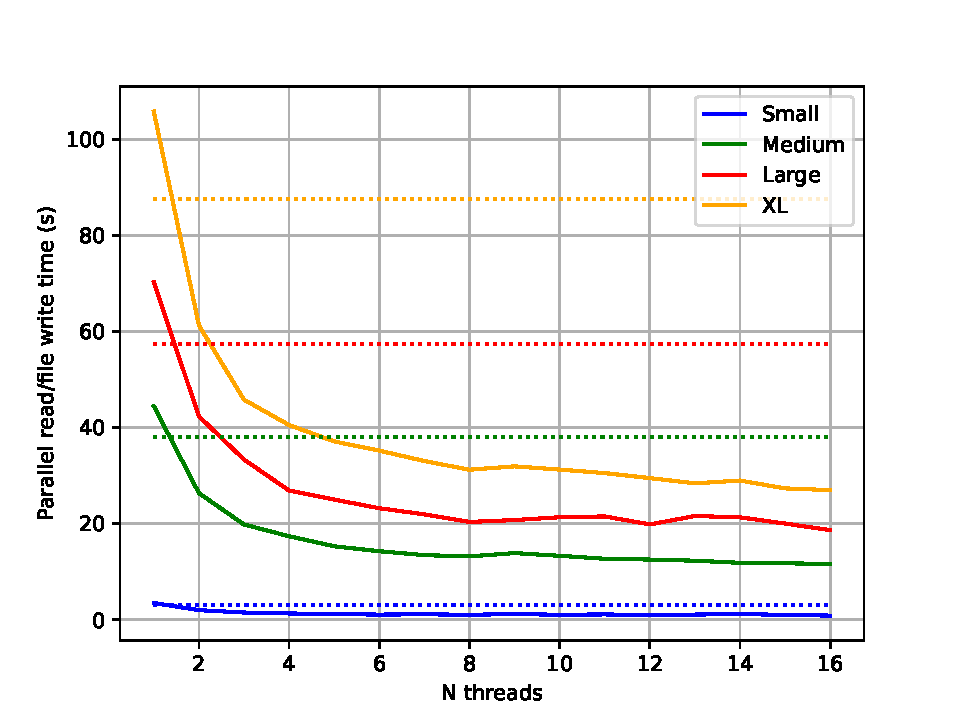
\includegraphics[width=\linewidth]{figs/cores.pdf}
    \label{fig:cores}
    \caption{Time to read differently-sized FASTQ \gzip files using a pre-built
    index file and different numbers of threads. Time compasses total program
    execution, including reading the index files, parallel reading the \gzip
    file with $N$ threads, and writing the reconstituted file to disk. Time for
    \texttt{zcat} to read the file and write it to disk is shown for comparison
    using a dotted line (\texttt{zcat} execution is single threaded). See
    Table~\ref{tab:source} for descriptions of small, medium, large, and XL.}
\end{figure}

Using the index files we generated for each 


